%!TEX root = bertinR.tex
%$HeadURL: svn+ssh://gsawitzki@svn.r-forge.r-project.org/svnroot/bertin/pkg/inst/doc/bertinR.Rnw $
%$Id: bertinR.Rnw 82 2013-05-15 16:29:57Z gsawitzki $
%$Author: gsawitzki $

%\VignetteIndexEntry{Bertin Matrices}
%\VignetteIndexEntry{Bertin implementation}
%$HeadURL: svn+ssh://gsawitzki@svn.r-forge.r-project.org/svnroot/bertin/pkg/inst/doc/bertinR.Rnw $

% svn propset svn:keywords "Date Author Id Revision HeadURL URL" bertinR.Rnw
% setwd("/Users/gs/projects/rforge/bertin/pkg/bertin/inst/doc/")
%
%
% enc <- options(width = 56);  Sweave("bertinR.Rnw",output="bertinR.tex", keep.source=TRUE, eps = FALSE); options(enc)
% enc <- options(width = 56);  Sweave("bertinR.Rnw",output="bertinR.tex", keep.source=TRUE, debug = TRUE, eps = FALSE, encoding="utf8"); options(enc)


%	The help pages for RweaveLatex and Rtangle list the options supported by the default
%	Sweave and Stangle drivers.
%	%
%%  # en c <- options(en coding = "Mac Roman", width = 56)
%   install.packages(pkgs="/Users/gs/projects/rforge/bertin/bertin_0.1-52.tar.gz", type="source", repos=NULL)
% \usepackage{Sweave}
%global flags for conditional builds
%:flags
%\def\private{true}% comment out for public version
\listfiles

\def\solutions{true}% comment out to hide solutions
\def\usehyperref{true}% comment out to skip hyperref

\ifx\pdfoutput\undefined % We're not running pdftex
\documentclass[nogin, dvips,12pt,a4paper,twoside]{amsart}
\else
%\documentclass[pdftex,12pt,a4paper,twoside]{amsbook}
\documentclass[nogin, pdftex,12pt,a4paper,twoside]{amsart}
\usepackage{thumbpdf}
\pdfcompresslevel=9
\fi
%\usepackage[nogin]{Sweave}

\AtBeginDocument{\setkeys{Gin}{width=1.0\textwidth}}

\def\private{true}% comment out for public version

\usepackage{graphicx}
%\DeclareGraphicsRule{.tif}{png}{.png}{`convert #1 `dirname #1`/`basename #1 .tif`.png}
\usepackage[english]{babel}%hyphenation must be after babel
\usepackage[utf8]{inputenc}%applemac
\usepackage{svninfo}

%%for debugging:
%\usepackage{showidx}%show index entries per page
%\usepackage{showkeys}%show label, ref and cite keys. Supersedes showlabels

\usepackage{gssda}
\usepackage{bertinR}

\usepackage{amsfonts}
\usepackage[author-year]{amsrefs}
\usepackage{color}


%:layout parameters
\setlength{\parskip}{12pt}
\setlength{\parindent}{0pt}
%! ?? undefined
%\setkeys{Gin}{width=0.9\textwidth}

%\author{G\"unther Sawitzki\\StatLab Heidelberg
%\\\bigskip\bigskip\today
%\bigskip\bigskip \\  \emph{\textcolor{red}{in preparation}}  %?? red undefined ?
%\bigskip\bigskip\bigskip\bigskip\bigskip \\  \emph{http://bertin-forge.r-project.org/}
%}

%:title
\title[Bertin Matrices]{Bertin Matrices\\\bigskip An\  \Rlogo \  Implementation}
%
\author[G\"unther Sawitzki]{G\"unther Sawitzki\\StatLab Heidelberg}
%	\contrib[...]{...} no2 |
\address{Address: G. Sawitzki, StatLab Heidelberg, Im Neuenheimer Feld 294, D 69120 Heidelberg}
%	\curraddr{...} no no
\email{gs@statlab.uni-heidelberg.de}
\urladdr{http://bertin.r-forge.r-project.org/}
%\dedicatory{in preparation}

\date{Aug. 2010.
%\svnInfoFile \svnInfoRevision
%For quotation, please use the general reference \cite{gs94oned}.\\
\emph{Revised:} August 2011\\
\emph{Typeset}, with minor revisions: \today\  from SVN $Revision: 82 $ \svnInfoDate}  
\thanks{\emph{URL:} \url{http://bertin. r-forge.r-project.org/}}
%	\translator{...} |3 |3
\keywords{statistical computing, S~programming language, R~programming,
data analysis, exploratory statistics, residual diagnostics, R language}
%\date{Aug. 2010, published as technical report \cite{gs92shrth}.\\
%	\subjclass[2000]{...} yes yes
%	\begin{abstract}...\end{abstract} yes4 no

%see: http://theoval.cmp.uea.ac.uk/~nlct/latex/pdfdoc/pdfdoc/pdfdoc.html
\pdfinfo{
   /Author (G. Sawitzki)
   /Title  (Bertin Matrices  - An R Implementation)
   /Subject (Computational Statistics)
   /Keywords (computational statistics, statistical computing, S~programming language, R~programming,
data analysis, exploratory statistics, Bertin, R~language)
}

%%for debugging:
%\usepackage{showidx}%show index entries per page
%\usepackage{showkeys}%show label, ref and cite keys. Supersedes showlabels
%
%%toc upto section level
%\setcounter{tocdepth}{2}
%\setcounter{secnumdepth}{4}
\makeindex

%:\begin{document}
\begin{document}
inst/doc

\svnInfo $Id: bertinR.Rnw 82 2013-05-15 16:29:57Z gsawitzki $ 

\svninfo $HeadURL: svn+ssh://gsawitzki@svn.r-forge.r-project.org/svnroot/bertin/pkg/inst/doc/bertinR.Rnw $
%\setkeys{Gin}{width=1.0\textwidth}
\maketitle

\begingroup
\setlength{\parskip}{0pt}
\tableofcontents
\endgroup

\section{Bertin Plots}
\setkeys{Gin}{width=1.0\textwidth}

Among the rich material on graphical presentation of information, in \cite{brtn77gtg}, engl. \cite{seriation:Bertin:1999}, J. Bertin discusses the presentation of data matrices, with a particular view to seriation. \cite{seriation:Falguerolles:1997} gives an appraisal of this aspect of Bertin's work. The methods discussed in \cite{seriation:Falguerolles:1997} have been implemented in the Voyager system \cite{Sawitzki1996Extensible-Stat}. They have been partially re-implemented in \R{}, and this paper gives an introduction to the \R{} implementation.

The \R{}-implementation can be downloaded as a package \ircode{bertin} from \url{http://bertin.r-forge.r-project.org/}.  The paper \cite{seriation:Falguerolles:1997} is included as bertin.pdf in the documentation section of the package.

Bertin uses a small data set on hotel occupancy data to illustrate his ideas.

%:  Hotel Data
\begin{table}[htdp]
\begin{center}%\leftskip-2em
%\begin{table}
\tiny{
\begin{tabular}{|l|r|r|r|r|r|r|r|r|r|r|r|r|}
\hline
&Jan&Fev&Mars&Avril&May&Juin&Juil&Aout&Sept&Oct&Nov&Dec\\
\hline
ClienteleFeminine&26&21&26&28&20&20&20&20&20&40&15&40\\
Locale&69&70&77&71&37&36&39&39&55&60&68&72\\
USA&7&6&3&6&23&14&19&14&9&6&8&8\\
AmerSud&0&0&0&0&8&6&6&4&2&12&0&0\\
Europe&20&15&14&15&23&27&22&30&27&19&19&17\\
MOrientAfrique&1&0&0&8&6&4&6&4&2&1&0&1\\
Asie&3&10&6&0&3&13&8&9&5&2&5&2\\
Business&78&80&85&86&85&87&70&76&87&85&87&80\\
Touristes&22&20&15&14&15&13&30&24&13&15&13&20\\
ResDirecte&70&70&78&74&69&68&74&75&68&68&64&75\\
ResAgents&20&18&19&17&27&27&19&19&26&27&21&15\\
EquipageAeriens&10&12&6&9&4&5&7&6&6&5&15&10\\
MoinsDe20&2&2&4&2&2&1&1&2&2&4&2&5\\
De20a55&25&27&37&35&25&25&27&28&24&30&24&30\\
De35a55&48&49&42&48&54&55&53&51&55&46&55&43\\
PlusDe55&25&22&17&15&19&19&19&19&19&20&19&22\\
Prix&163&167&166&174&152&155&145&170&157&174&165&156\\
Duree&1.65&1.71&1.65&1.91&1.9&2&1.54&1.6&1.73&1.82&1.66&1.44\\
Occupation&67&82&70&83&74&77&56&62&90&92&78&55\\
Foires&0&0&0&1&1&1&0&0&1&1&1&1\\
\hline
\end{tabular}
}
%\caption{Bertin's Hotel data}
%\end{table}
\end{center}
\caption{Bertin's hotel data}
\label{tab:hotel}
\end{table}%

\section{Bertin Matrices}

To repeat from  \cite{seriation:Falguerolles:1997}: In abstract terms, a Bertin matrix is a matrix of displays. Bertin matrices allow rearrangements to
transform an initial matrix to a more homogeneous structure. The rearrangements are row or column
permutations, and groupings of rows or columns. To fix ideas, think of a data matrix, variable by
case, with real valued variables. For each variable, draw a bar chart of variable value by case. Highlight
all bars representing a value above some sample threshold for that variable (\reffig{fig:hotel19}).


%: fig 01 hotel19
\begin{figure}[htbp]
\begin{center}
\includegraphics[width=0.9\linewidth]{"bertinR-hotel19"}
\caption{Display of one variable: \textbf{Hotel data}.  Observations above average are highlighted in black.}
\label{fig:hotel19}
\end{center}
\end{figure}

Variables are collected in a matrix to display the complete data set (\reffig{fig:hotelorig}). By convention, Bertin shows variables in rows and cases in columns. To make periodic structures more visible, the data are  repeated cyclically.

%<<fig=TRUE, include = FALSE, echo=FALSE, label=hotelorig, width=5, height=4>>=

%: fig 02 hotelorig
\begin{figure}[htbp]
\begin{center}
\includegraphics[width=1.0\linewidth]{"bertinR-hotelorig"}
\caption{Display of a data matrix: \textbf{Hotel data}. Variables are shown as rows. To make periodic structures more visible, time is duplicated. Observations above average are highlighted.}
\label{fig:hotelorig}
\end{center}
\end{figure}

As Bertin points out, the indexing used is arbitrary. You can rearrange rows and/or columns to reveal the information of interest. If you run a hotel, of course the percentage of hotel occupation and the duration of the visits are most interesting for you. Move these variables to the top of the display, and rearrange the other variables by similarity or dissimilarity to these target variables (\reffig{fig:hotelperm}). Time points have a natural order. No rearrangement is used here.

%: fig 03 hotelperm
%<<fig=TRUE, include = FALSE, echo=FALSE, label=hotelperm, width=8, height=5>>=
%colmeans <- apply(Hotel2,1,mean)
%rowperm <- c(19,18,20, 8, 11, 4, 12, 13,16,14,1,2, 7, 9, 10, 17, 6, 3, 5,15)
%col=ifelse(Hotel2[,]>colmeans, "black","white")
%bertinrect(Hotel2[rowperm,], main="Hotel 2", 
%	col=col[rowperm,],  pars = list(mar=c(0.2,0.2,4,8)))
%	title(sub="Variables rearranged")
%abline(h=7.1, col= "green", lwd=3)
%abline(h=11.5, col= "green", lwd=3)
%abline(h=14.3, col= "green", lwd=3)
%@

%
\begin{figure}[htbp]
\begin{center}
\includegraphics[width=1.0\linewidth]{"bertinR-hotelperm"}
\caption{Display of a data matrix: \textbf{Hotel data}. Variables are rearranged by similarity to occupation and duration.}
\label{fig:hotelperm}
\end{center}
\end{figure}

Variables need not enter at their face value; they can be transformed, or derived variable can be added. In the case of the hotel data, this has already done in the original data set. For example, the guests have been classified in tourists and business, and both sum up to 100\%.  If we want, we can remove this redundant information. This may clean up the picture. But it may hide information. For example, $tourists$ are ``anti-cyclic'' to the hotel occupation and just fill the gaps. Removing this variable because it is $(1-business)$ would hide this point.
%! clean up. Fix data for 100% sums. Fix age groups.


%
\begin{figure}[htbp]
\begin{center}
\includegraphics[width=1.0\linewidth]{"bertinR-hotelperm1"}
\caption{Display of a data matrix: \textbf{Hotel data}. Variables are rearranged by similarity to occupation and duration. Some redundancy removed.}
\label{fig:hotelperm1}
\end{center}
\end{figure}

\clearpage
As a second example, we use the  the \ircode{USJudgeRatings} data set (\reffig{fig:judgeorig}). 
The data  is listed in  \reftab{tab:judge}.
%<<results=tex, echo=FALSE, include=FALSE>>=
%print(xtable(USJudgeRatings,label="tab:judge", caption="US judge ratings"), floating=TRUE)
%@

%	%\begin{minipage}{0.6\linewidth}
%	\begin{table}[ht]
%	\begin{center}
%	\tiny{
%	\begin{tabular}{rrrrrrrrrrrrr}
%	 \hline
%	&CONT&INTG&DMNR&DILG&CFMG&DECI&PREP&FAMI&ORAL&WRIT&PHYS&RTEN\\
%	 \hline
%	AAR,L.H.&5.7&7.9&7.7&7.3&7.1&7.4&7.1&7.1&7.1&7.0&8.3&7.80 \\ 
%	ALE,J.M.&6.8&8.9&8.8&8.5&7.8&8.1&8.0&8.0&7.8&7.9&8.5&8.7\\ 
%	ARM,A.J.&7.2&8.1&7.8&7.8&7.5&7.6&7.5&7.5&7.3&7.4&7.9&7.8\\ 
%	BER,R.I.&6.8&8.8&8.5&8.8&8.3&8.5&8.7&8.7&8.4&8.5&8.8&8.7\\ 
%	BRA,J.J.&7.3&6.4&4.3&6.5&6.0&6.2&5.7&5.7&5.1&5.3&5.5&4.8\\ 
%	BUR,E.B.&6.2&8.8&8.7&8.5&7.9&8.0&8.1&8.0&8.0&8.0&8.6&8.6\\ 
%	CAL,R.J.&10.6&9.0&8.9&8.7&8.5&8.5&8.5&8.5&8.6&8.4&9.1&9.0\\ 
%	COH,S.S.&7.0&5.9&4.9&5.1&5.4&5.9&4.8&5.1&4.7&4.9&6.8&5.0\\ 
%	DAL,J.J.&7.3&8.9&8.9&8.7&8.6&8.5&8.4&8.4&8.4&8.5&8.8&8.8\\ 
%	DAN,J.F.&8.2&7.9&6.7&8.1&7.9&8.0&7.9&8.1&7.7&7.8&8.5&7.9\\ 
%	DEA,H.H.&7.0&8.0&7.6&7.4&7.3&7.5&7.1&7.2&7.1&7.2&8.4&7.7\\ 
%	DEV,H.J.&6.5&8.0&7.6&7.2&7.0&7.1&6.9&7.0&7.0&7.1&6.9&7.2\\ 
%	DRI,P.J.&6.7&8.6&8.2&6.8&6.9&6.6&7.1&7.3&7.2&7.2&8.1&7.7\\ 
%	GRI,A.E.&7.0&7.5&6.4&6.8&6.5&7.0&6.6&6.8&6.3&6.6&6.2&6.5\\ 
%	HAD,W.L.JR.&6.5&8.1&8.0&8.0&7.9&8.0&7.9&7.8&7.8&7.8&8.4&8.0\\ 
%	HAM,E.C.&7.3&8.0&7.4&7.7&7.3&7.3&7.3&7.2&7.1&7.2&8.0&7.6\\ 
%	HEA,A.H.&8.0&7.6&6.6&7.2&6.5&6.5&6.8&6.7&6.4&6.5&6.9&6.7\\ 
%	HUL,T.C.&7.7&7.7&6.7&7.5&7.4&7.5&7.1&7.3&7.1&7.3&8.1&7.4\\ 
%	LEV,I.&8.3&8.2&7.4&7.8&7.7&7.7&7.7&7.8&7.5&7.6&8.0&8.0\\ 
%	LEV,R.L.&9.6&6.9&5.7&6.6&6.9&6.6&6.2&6.0&5.8&5.8&7.2&6.0\\ 
%	MAR,L.F.&7.1&8.2&7.7&7.1&6.6&6.6&6.7&6.7&6.8&6.8&7.5&7.3\\ 
%	MCG,J.F.&7.6&7.3&6.9&6.8&6.7&6.8&6.4&6.3&6.3&6.3&7.4&6.6\\ 
%	MIG,A.F.&6.6&7.4&6.2&6.2&5.4&5.7&5.8&5.9&5.2&5.8&4.7&5.2\\ 
%	MISL,H.M.&6.2&8.3&8.1&7.7&7.4&7.3&7.3&7.3&7.2&7.3&7.8&7.6\\ 
%	MUL,H.M.&7.5&8.7&8.5&8.6&8.5&8.4&8.5&8.5&8.4&8.4&8.7&8.7\\ 
%	NAR,H.J.&7.8&8.9&8.7&8.9&8.7&8.8&8.9&9.0&8.8&8.9&9.0&9.0\\ 
%	O'BR,F.J.&7.1&8.5&8.3&8.0&7.9&7.9&7.8&7.8&7.8&7.7&8.3&8.2\\ 
%	O'SU,T.J.&7.5&9.0&8.9&8.7&8.4&8.5&8.4&8.3&8.3&8.3&8.8&8.7\\ 
%	PAS,L.&7.5&8.1&7.7&8.2&8.0&8.1&8.2&8.4&8.0&8.1&8.4&8.1\\ 
%	RUB,J.E.&7.1&9.2&9.0&9.0&8.4&8.6&9.1&9.1&8.9&9.0&8.9&9.2\\ 
%	SAD.G.A.&6.6&7.4&6.9&8.4&8.0&7.9&8.2&8.4&7.7&7.9&8.4&7.5\\ 
%	SAT,A.G.&8.4&8.0&7.9&7.9&7.8&7.8&7.6&7.4&7.4&7.4&8.1&7.9\\ 
%	SHE,D.M.&6.9&8.5&7.8&8.5&8.1&8.2&8.4&8.5&8.1&8.3&8.7&8.3\\ 
%	SHE,J.F.JR.&7.3&8.9&8.8&8.7&8.4&8.5&8.5&8.5&8.4&8.4&8.8&8.8\\ 
%	SID,W.J.&7.7&6.2&5.1&5.6&5.6&5.9&5.6&5.6&5.3&5.5&6.3&5.3\\ 
%	SPE,J.A.&8.5&8.3&8.1&8.3&8.4&8.2&8.2&8.1&7.9&8.0&8.0&8.2\\ 
%	SPO,M.J.&6.9&8.3&8.0&8.1&7.9&7.9&7.9&7.7&7.6&7.7&8.1&8.0\\ 
%	STA,J.F.&6.5&8.2&7.7&7.8&7.6&7.7&7.7&7.7&7.5&7.6&8.5&7.7\\ 
%	TES,R.J.&8.3&7.3&7.0&6.8&7.0&7.1&6.7&6.7&6.7&6.7&8.0&7.0\\ 
%	TIE,W.L.JR.&8.3&8.2&7.8&8.3&8.4&8.3&7.7&7.6&7.5&7.7&8.1&7.9\\ 
%	WAL,R.A.&9.0&7.0&5.9&7.0&7.0&7.2&6.9&6.9&6.5&6.6&7.6&6.6\\ 
%	WRI,D.B.&7.1&8.4&8.4&7.7&7.5&7.7&7.8&8.2&8.0&8.1&8.3&8.1\\ 
%	ZAR,K.J.&8.6&7.4&7.0&7.5&7.5&7.7&7.4&7.2&6.9&7.0&7.8&7.1\\ 
%	  \hline
%	\end{tabular}
%	}
%	\caption{US judge ratings}
%	\label{tab:judge}
%	\end{center}
%	\end{table}
%	%\end{minipage}
%	
%:  USJudgeRatings Data
%\begin{minipage}\linewidth
\begin{table}[ht]
\begin{center}\tabcolsep0.2em%\leftskip-2em
\tiny{
\begin{tabular}{rrrrrrrrrrrrr}
\hline
& CONT&INTG&DMNR&DILG&CFMG&DECI&PREP&FAMI&ORAL&WRIT&PHYS&RTEN \\ 
\hline
AAR,L.H.&5.7&7.9&7.7&7.3&7.1&7.4&7.1&7.1&7.1&7.0&8.3&7.80 \\ 
ALE,J.M.&6.8&8.9&8.8&8.5&7.8&8.1&8.0&8.0&7.8&7.9&8.5&8.7\\ 
ARM,A.J.&7.2&8.1&7.8&7.8&7.5&7.6&7.5&7.5&7.3&7.4&7.9&7.8\\ 
BER,R.I.&6.8&8.8&8.5&8.8&8.3&8.5&8.7&8.7&8.4&8.5&8.8&8.7\\ 
BRA,J.J.&7.3&6.4&4.3&6.5&6.0&6.2&5.7&5.7&5.1&5.3&5.5&4.8\\ 
BUR,E.B.&6.2&8.8&8.7&8.5&7.9&8.0&8.1&8.0&8.0&8.0&8.6&8.6\\ 
CAL,R.J.&10.6&9.0&8.9&8.7&8.5&8.5&8.5&8.5&8.6&8.4&9.1&9.0\\ 
COH,S.S.&7.0&5.9&4.9&5.1&5.4&5.9&4.8&5.1&4.7&4.9&6.8&5.0\\ 
DAL,J.J.&7.3&8.9&8.9&8.7&8.6&8.5&8.4&8.4&8.4&8.5&8.8&8.8\\ 
DAN,J.F.&8.2&7.9&6.7&8.1&7.9&8.0&7.9&8.1&7.7&7.8&8.5&7.9\\ 
DEA,H.H.&7.0&8.0&7.6&7.4&7.3&7.5&7.1&7.2&7.1&7.2&8.4&7.7\\ 
DEV,H.J.&6.5&8.0&7.6&7.2&7.0&7.1&6.9&7.0&7.0&7.1&6.9&7.2\\ 
DRI,P.J.&6.7&8.6&8.2&6.8&6.9&6.6&7.1&7.3&7.2&7.2&8.1&7.7\\ 
GRI,A.E.&7.0&7.5&6.4&6.8&6.5&7.0&6.6&6.8&6.3&6.6&6.2&6.5\\ 
HAD,W.L.JR.&6.5&8.1&8.0&8.0&7.9&8.0&7.9&7.8&7.8&7.8&8.4&8.0\\ 
HAM,E.C.&7.3&8.0&7.4&7.7&7.3&7.3&7.3&7.2&7.1&7.2&8.0&7.6\\ 
HEA,A.H.&8.0&7.6&6.6&7.2&6.5&6.5&6.8&6.7&6.4&6.5&6.9&6.7\\ 
HUL,T.C.&7.7&7.7&6.7&7.5&7.4&7.5&7.1&7.3&7.1&7.3&8.1&7.4\\ 
LEV,I.&8.3&8.2&7.4&7.8&7.7&7.7&7.7&7.8&7.5&7.6&8.0&8.0\\ 
LEV,R.L.&9.6&6.9&5.7&6.6&6.9&6.6&6.2&6.0&5.8&5.8&7.2&6.0\\ 
MAR,L.F.&7.1&8.2&7.7&7.1&6.6&6.6&6.7&6.7&6.8&6.8&7.5&7.3\\ 
MCG,J.F.&7.6&7.3&6.9&6.8&6.7&6.8&6.4&6.3&6.3&6.3&7.4&6.6\\ 
MIG,A.F.&6.6&7.4&6.2&6.2&5.4&5.7&5.8&5.9&5.2&5.8&4.7&5.2\\ 
MISL,H.M.&6.2&8.3&8.1&7.7&7.4&7.3&7.3&7.3&7.2&7.3&7.8&7.6\\ 
MUL,H.M.&7.5&8.7&8.5&8.6&8.5&8.4&8.5&8.5&8.4&8.4&8.7&8.7\\ 
NAR,H.J.&7.8&8.9&8.7&8.9&8.7&8.8&8.9&9.0&8.8&8.9&9.0&9.0\\ 
O'BR,F.J.&7.1&8.5&8.3&8.0&7.9&7.9&7.8&7.8&7.8&7.7&8.3&8.2\\ 
O'SU,T.J.&7.5&9.0&8.9&8.7&8.4&8.5&8.4&8.3&8.3&8.3&8.8&8.7\\ 
PAS,L.&7.5&8.1&7.7&8.2&8.0&8.1&8.2&8.4&8.0&8.1&8.4&8.1\\ 
RUB,J.E.&7.1&9.2&9.0&9.0&8.4&8.6&9.1&9.1&8.9&9.0&8.9&9.2\\ 
SAD.G.A.&6.6&7.4&6.9&8.4&8.0&7.9&8.2&8.4&7.7&7.9&8.4&7.5\\ 
SAT,A.G.&8.4&8.0&7.9&7.9&7.8&7.8&7.6&7.4&7.4&7.4&8.1&7.9\\ 
SHE,D.M.&6.9&8.5&7.8&8.5&8.1&8.2&8.4&8.5&8.1&8.3&8.7&8.3\\ 
SHE,J.F.JR.&7.3&8.9&8.8&8.7&8.4&8.5&8.5&8.5&8.4&8.4&8.8&8.8\\ 
SID,W.J.&7.7&6.2&5.1&5.6&5.6&5.9&5.6&5.6&5.3&5.5&6.3&5.3\\ 
SPE,J.A.&8.5&8.3&8.1&8.3&8.4&8.2&8.2&8.1&7.9&8.0&8.0&8.2\\ 
SPO,M.J.&6.9&8.3&8.0&8.1&7.9&7.9&7.9&7.7&7.6&7.7&8.1&8.0\\ 
STA,J.F.&6.5&8.2&7.7&7.8&7.6&7.7&7.7&7.7&7.5&7.6&8.5&7.7\\ 
TES,R.J.&8.3&7.3&7.0&6.8&7.0&7.1&6.7&6.7&6.7&6.7&8.0&7.0\\ 
TIE,W.L.JR.&8.3&8.2&7.8&8.3&8.4&8.3&7.7&7.6&7.5&7.7&8.1&7.9\\ 
WAL,R.A.&9.0&7.0&5.9&7.0&7.0&7.2&6.9&6.9&6.5&6.6&7.6&6.6\\ 
WRI,D.B.&7.1&8.4&8.4&7.7&7.5&7.7&7.8&8.2&8.0&8.1&8.3&8.1\\ 
ZAR,K.J.&8.6&7.4&7.0&7.5&7.5&7.7&7.4&7.2&6.9&7.0&7.8&7.1\\ 
%AARONSON,L.H.&5.70&7.90&7.70&7.30&7.10&7.40&7.10&7.10&7.10&7.00&8.30&7.80 \\ 
%ALEXANDER,J.M.&6.80&8.90&8.80&8.50&7.80&8.10&8.00&8.00&7.80&7.90&8.50&8.70 \\ 
%ARMENTANO,A.J.&7.20&8.10&7.80&7.80&7.50&7.60&7.50&7.50&7.30&7.40&7.90&7.80 \\ 
%BERDON,R.I.&6.80&8.80&8.50&8.80&8.30&8.50&8.70&8.70&8.40&8.50&8.80&8.70 \\ 
%BRACKEN,J.J.&7.30&6.40&4.30&6.50&6.00&6.20&5.70&5.70&5.10&5.30&5.50&4.80 \\ 
%BURNS,E.B.&6.20&8.80&8.70&8.50&7.90&8.00&8.10&8.00&8.00&8.00&8.60&8.60 \\ 
%CALLAHAN,R.J.&10.60&9.00&8.90&8.70&8.50&8.50&8.50&8.50&8.60&8.40&9.10&9.00 \\ 
%COHEN,S.S.&7.00&5.90&4.90&5.10&5.40&5.90&4.80&5.10&4.70&4.90&6.80&5.00 \\ 
%DALY,J.J.&7.30&8.90&8.90&8.70&8.60&8.50&8.40&8.40&8.40&8.50&8.80&8.80 \\ 
%DANNEHY,J.F.&8.20&7.90&6.70&8.10&7.90&8.00&7.90&8.10&7.70&7.80&8.50&7.90 \\ 
%DEAN,H.H.&7.00&8.00&7.60&7.40&7.30&7.50&7.10&7.20&7.10&7.20&8.40&7.70 \\ 
%DEVITA,H.J.&6.50&8.00&7.60&7.20&7.00&7.10&6.90&7.00&7.00&7.10&6.90&7.20 \\ 
%DRISCOLL,P.J.&6.70&8.60&8.20&6.80&6.90&6.60&7.10&7.30&7.20&7.20&8.10&7.70 \\ 
%GRILLO,A.E.&7.00&7.50&6.40&6.80&6.50&7.00&6.60&6.80&6.30&6.60&6.20&6.50 \\ 
%HADDEN,W.L.JR.&6.50&8.10&8.00&8.00&7.90&8.00&7.90&7.80&7.80&7.80&8.40&8.00 \\ 
%HAMILL,E.C.&7.30&8.00&7.40&7.70&7.30&7.30&7.30&7.20&7.10&7.20&8.00&7.60 \\ 
%HEALEY.A.H.&8.00&7.60&6.60&7.20&6.50&6.50&6.80&6.70&6.40&6.50&6.90&6.70 \\ 
%HULL,T.C.&7.70&7.70&6.70&7.50&7.40&7.50&7.10&7.30&7.10&7.30&8.10&7.40 \\ 
%LEVINE,I.&8.30&8.20&7.40&7.80&7.70&7.70&7.70&7.80&7.50&7.60&8.00&8.00 \\ 
%LEVISTER,R.L.&9.60&6.90&5.70&6.60&6.90&6.60&6.20&6.00&5.80&5.80&7.20&6.00 \\ 
%MARTIN,L.F.&7.10&8.20&7.70&7.10&6.60&6.60&6.70&6.70&6.80&6.80&7.50&7.30 \\ 
%MCGRATH,J.F.&7.60&7.30&6.90&6.80&6.70&6.80&6.40&6.30&6.30&6.30&7.40&6.60 \\ 
%MIGNONE,A.F.&6.60&7.40&6.20&6.20&5.40&5.70&5.80&5.90&5.20&5.80&4.70&5.20 \\ 
%MISSAL,H.M.&6.20&8.30&8.10&7.70&7.40&7.30&7.30&7.30&7.20&7.30&7.80&7.60 \\ 
%MULVEY,H.M.&7.50&8.70&8.50&8.60&8.50&8.40&8.50&8.50&8.40&8.40&8.70&8.70 \\ 
%NARUK,H.J.&7.80&8.90&8.70&8.90&8.70&8.80&8.90&9.00&8.80&8.90&9.00&9.00 \\ 
%O'BRIEN,F.J.&7.10&8.50&8.30&8.00&7.90&7.90&7.80&7.80&7.80&7.70&8.30&8.20 \\ 
%O'SULLIVAN,T.J.&7.50&9.00&8.90&8.70&8.40&8.50&8.40&8.30&8.30&8.30&8.80&8.70 \\ 
%PASKEY,L.&7.50&8.10&7.70&8.20&8.00&8.10&8.20&8.40&8.00&8.10&8.40&8.10 \\ 
%RUBINOW,J.E.&7.10&9.20&9.00&9.00&8.40&8.60&9.10&9.10&8.90&9.00&8.90&9.20 \\ 
%SADEN.G.A.&6.60&7.40&6.90&8.40&8.00&7.90&8.20&8.40&7.70&7.90&8.40&7.50 \\ 
%SATANIELLO,A.G.&8.40&8.00&7.90&7.90&7.80&7.80&7.60&7.40&7.40&7.40&8.10&7.90 \\ 
%SHEA,D.M.&6.90&8.50&7.80&8.50&8.10&8.20&8.40&8.50&8.10&8.30&8.70&8.30 \\ 
%SHEA,J.F.JR.&7.30&8.90&8.80&8.70&8.40&8.50&8.50&8.50&8.40&8.40&8.80&8.80 \\ 
%SIDOR,W.J.&7.70&6.20&5.10&5.60&5.60&5.90&5.60&5.60&5.30&5.50&6.30&5.30 \\ 
%SPEZIALE,J.A.&8.50&8.30&8.10&8.30&8.40&8.20&8.20&8.10&7.90&8.00&8.00&8.20 \\ 
%SPONZO,M.J.&6.90&8.30&8.00&8.10&7.90&7.90&7.90&7.70&7.60&7.70&8.10&8.00 \\ 
%STAPLETON,J.F.&6.50&8.20&7.70&7.80&7.60&7.70&7.70&7.70&7.50&7.60&8.50&7.70 \\ 
%TESTO,R.J.&8.30&7.30&7.00&6.80&7.00&7.10&6.70&6.70&6.70&6.70&8.00&7.00 \\ 
%TIERNEY,W.L.JR.&8.30&8.20&7.80&8.30&8.40&8.30&7.70&7.60&7.50&7.70&8.10&7.90 \\ 
%WALL,R.A.&9.00&7.00&5.90&7.00&7.00&7.20&6.90&6.90&6.50&6.60&7.60&6.60 \\ 
%WRIGHT,D.B.&7.10&8.40&8.40&7.70&7.50&7.70&7.80&8.20&8.00&8.10&8.30&8.10 \\ 
%ZARRILLI,K.J.&8.60&7.40&7.00&7.50&7.50&7.70&7.40&7.20&6.90&7.00&7.80&7.10 \\ 
\hline
\end{tabular}
}
\caption{US judge ratings}
\label{tab:judge}
\end{center}
\end{table}
%\end{minipage}

%: fig04 judgeorig



\begin{figure}[htbp]
\begin{center}
\includegraphics[width=1.0\linewidth]{"bertinR-judgeorig"}
\caption{Display of a data matrix: \textbf{USJudgeRatings data}. Lawyers' ratings of state judges in the US Superior Court. Original arrangement, judges by lexical order of name.}
\label{fig:judgeorig}
\end{center}
\end{figure}

Both the cases (the judges) and the variables (the qualities) allow for a rearrangement. Just sorting for row and column averages gives a more informative picture  (\reffig{fig:judgeperm}). The number of contacts \ircode{CONT} stands out - it has a different structure than the other variables. After all, this is not a rating variable at all, but ancillary information. There is little reason why it should go along with the rating variables. Judge G.~A.~Saden seems to be special. Most variables would rank him to the upper group, be his worth of retention is below average. The esteem of his integrity and demeanour go along with this. Overall, there is a very clear separation into an upper and a lower group.



%: fig05 judgeperm
%
\begin{figure}[htbp]
\begin{center}
\includegraphics[width=1.0\linewidth]{"bertinR-judgeperm"}
\caption{Display of a data matrix. \textbf{USJudgeRatings data}. Lawyers' ratings of state judges in the US Superior Court, rearranged.}
\label{fig:judgeperm}
\end{center}
\end{figure}

We remove the variable \ircode{CONT} and re-run the analysis. Of course this changes the average scores per judge, and the arrangement changes (\reffig{fig:judgeperm1}).

\begin{figure}[htbp]
\begin{center}
\includegraphics[width=1.0\linewidth]{"bertinR-judgeperm1"}
\caption{Display of a data matrix. \textbf{USJudgeRatings data} Lawyers' ratings of state judges in the US Superior Court. Variable \ircode{CONT} removed, and rearranged.}
\label{fig:judgeperm1}
\end{center}
\end{figure}

The highlight features of the  display give a clear picture of a rather homogeneous upper and homogeneous lower group of judges. All criteria seem to say the same in these groups. For a small intermediate group of cases, the variables seem to fall into two or three groups, and it is only for this small group that a closer look at the variables and their meaning may be necessary. 
 If you want to model the rating of the worthiness of retention, say, as a function of the other ratings, it is only here that a refined model might be necessary. For most judges, a rough model would do.
 
 For this data set, the low resolution of the variables may be a problem. No details are given in the documentation, but  presumably the rating has been taken on a $1, \ldots, 10$ scale, and in all variables the median is higher than $7$. (only one data point, a contact recorded as 10.6 does not fit into this and asks for explanation.) Changing the scale may give a better contrast and improves the resolution (see \reffig{fig:judgeperm1rng}).  Here we used the rescaled variables to define the height of the bars. For highlighting by colour (only black/white here) we used the data in the original scale. Both display attributes, height and colour, are independent and we are free to encode different aspects of the data. In  \reffig{fig:judgeperm1rng} we sorted the cases by the value of \ircode{RTEN}. This lets us view the data from a different point of view.
 
Again we have a clear upper and lower group, with consistency over all variables, and a small intermediate group which needs closer inspection. Judge G.A. Saden stands out. By most criteria, he qualifies for a higher ranking, but demeanour and judicial integrity go along with a low scored worthy of retention.

Two judges are on the boundary and may well be exchanged - this is where random fluctuation may be at work to decide for the ranking.

\begin{figure}[htbp]
\begin{center}
\includegraphics{"bertinR-judgeperm1rng"}
\caption{Data set: \textbf{USJudgeRatings}. Cases sorted by RTEN, variables sorted by mean. Rescaled for range. CONT removed. Scores above mean are highlighted.}
\label{fig:judgeperm1rng}
\end{center}
\end{figure}

\clearpage
At this early point, let us put Bertin's work in place. Visualising information is but one aspect. In statistics, as we see it today, visualisation may be one part of an analysis. The outcome will be a decision leading to an action. Then there is a loss (or gain) depending on the action taken on the one hand, and the ``true'' state of the world on the other. This is the common decision theoretical setting. Statistics has formulated a few standard problems, and given suggestions how to handle these. In our Hotel example, the problem can be seen as a prediction problem: find a prediction model to predict occupation and duration, based on the other variables. More specifically this is a control problem, and the statistical contribution is to find a regression model for occupation and duration, based on the other variables. The visualisation can be seen as one way to hint at a regression model. There are very few classical problems. Regression is one of them, and prediction is closely related. Classification and clustering is another, closely related pair of problems, and their relation to Bertin matrices should be obvious. The USJudgeRatings can be looked at as a classification problem.


\section{Work flow}
\setkeys{Gin}{width=1.0\textwidth}

Bertin matrices usually are part of a work flow.

\begin{figure}[htbp]
\begin{center}
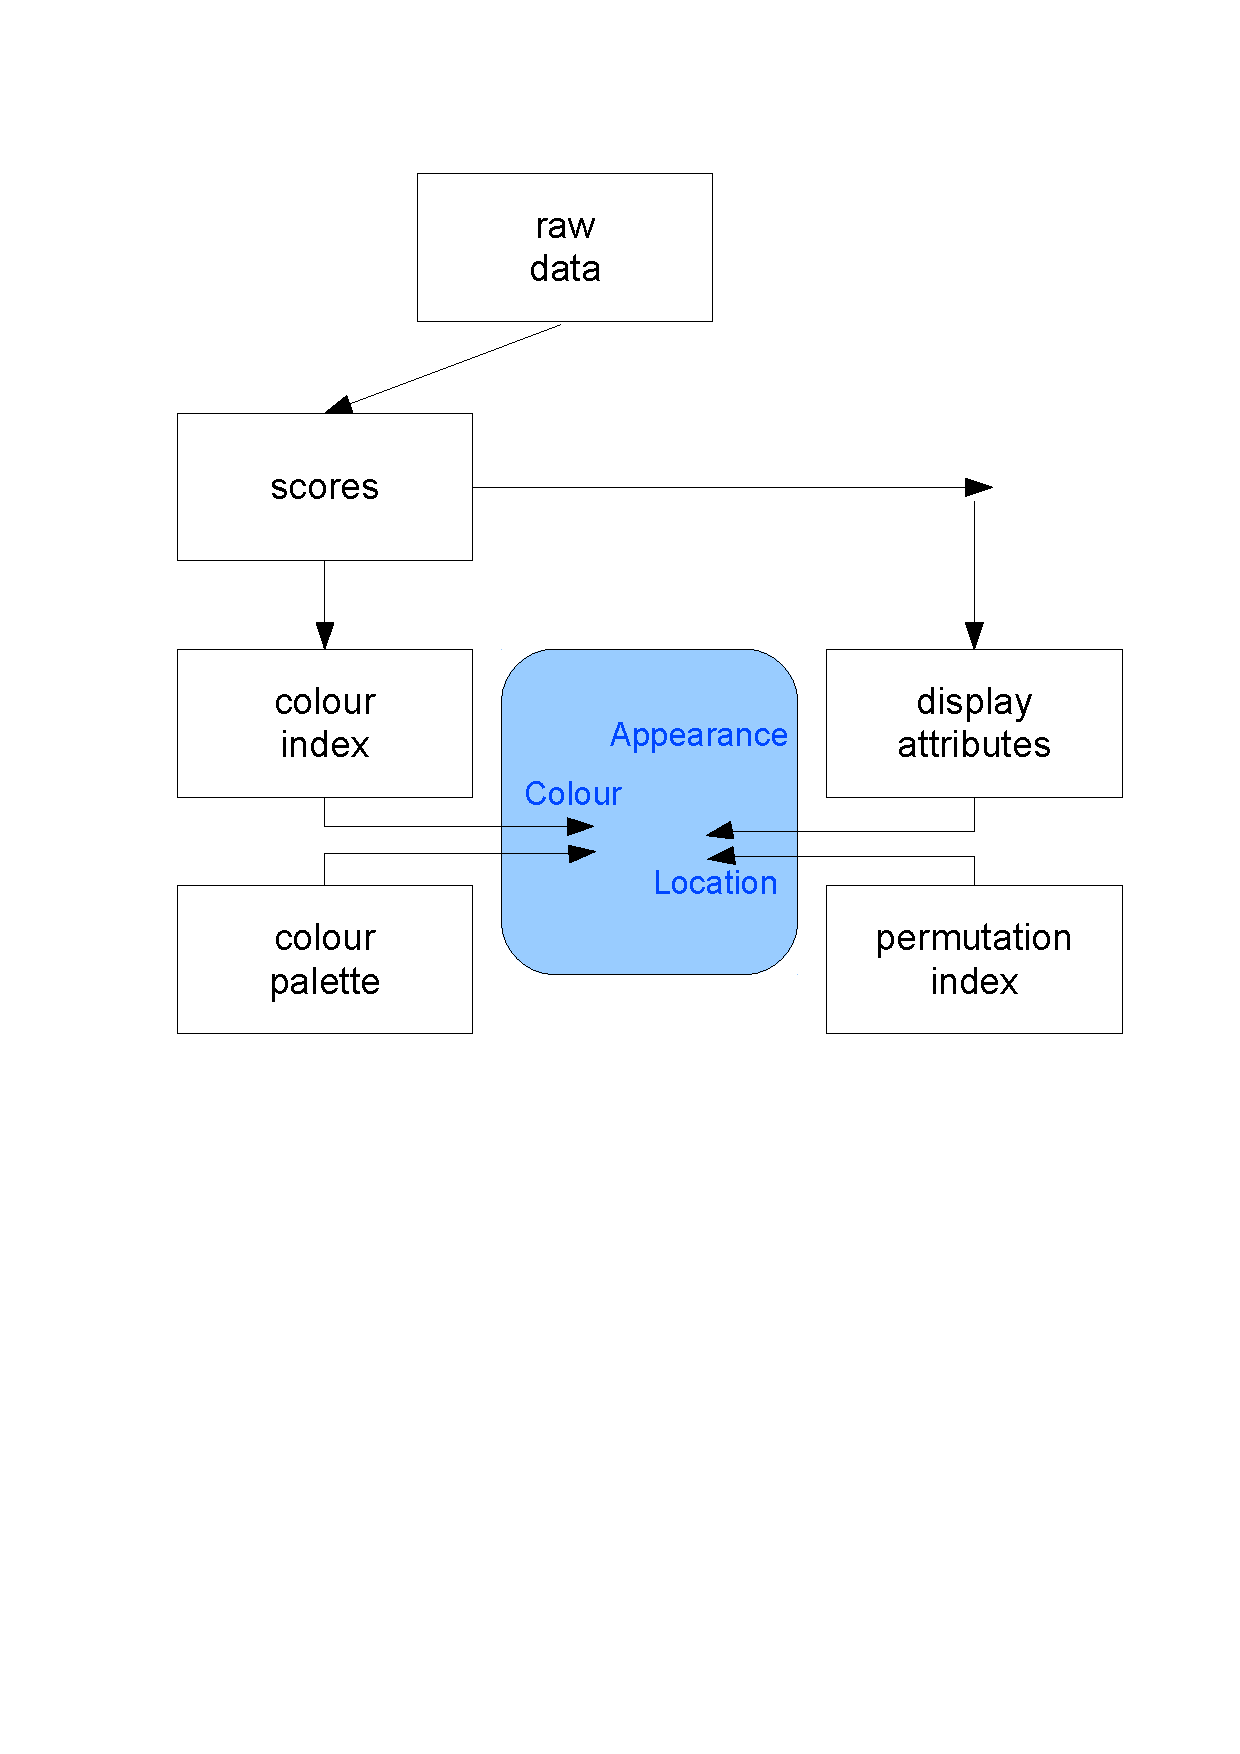
\includegraphics{workflow}
\caption{Data flow for Bertin}
\label{fig:workflow}
\end{center}
\end{figure}

In a first step, we transfer the input data to allow for  common, or comparable scales. In the Hotel example, Bertin rescales by the maximum value of each variable. The dichotomous variable Faires is encoded as 0/1. Our  implementation default is to rescale for  \ircode{(0, max)} for positive variables,  \ircode{(min, 0)} for negative variables,  \ircode{(min, max)} for general variables. Out preferred, or recommended rescaling however is to use ranks. We use the term \ircode{score} for the rescaled variables. Orientation of the data set is critical convention in this step. Usually, rescaling should be by variable, not by case. Depending on the orientation, this can lead for example to ranks by row or by column. We allow global scaling as an additional option for those situations where all data are already on a common scale. Following Bertin, our  implementation default is to expect variables in rows, but we provide the means to switch to the \R{} convention with variables in columns. The raw data may come in data frames, or lists, or views on a data base, and the original convention should be preserved. The scores however are a matrix, or an array (which we consider a stacked list of matrices in our context.) We prefer to keep these in Bertin conventions, that is variables are in rows.

In a second step, the scores are translated to visualisation attributes.  Colour is handled in two steps. The scores are translated to  a colour index, which is used together with a colour palette to determine the display colour for a data element. This allows rapid experiments with various colour palettes, as long as the length of the palettes are compatible. We strongly recommend to always look at the inverted colour palette together with a chosen one  to mitigate the effects of colour  perception. Simple image displays limit the  visualisation attributes to colour. \ircode{rect} for example allows rectangle geometry, colour, and border width. Shading and line types should be considered as an alternative for print media. 

Visualisation attributes may reflect different aspects. So for example in the classical Bertin display, height of a rectangle is used to reflect the value of a data element, colour is used to show an indicator whether the value is above or below variable mean.

A third step controls the actual placement of the graphical elements. With a matrix layout, it is specified by possible permutations of rows and of columns. This may be related to information used in the first two steps, but should be considered an independent step. A vector or row orders and of column orders is the critical information from this step. Various seriation methods apply. This is where Bertin's ideas about ``internal mobility''  as a characteristics of modern graphics come to action. The typical situation is to select scores and display attributes, and then search for optimal or good seriations. The arrangement often leads to hard optimisation problems. Placing this step later allows to use information from score transformation and attributes, which may allow more efficient algorithms. In the end, we may be better with a good solution which helps to solve the practical problem, instead of an optimal solution to a theoretical one. These may differ considerably.

The final step is to merge these informations and render a display. 

\section{Scores}
\setkeys{Gin}{width=1.0\textwidth}

In principle, scores can be generated using an appropriate score function and \ircode{apply} or any of its variants. 
As  examples, and for convenience, we provide a small collection of score functions. 

As an illustration, each is applied by row to the Hotel data set, and the result is shown using a default Bertin plot. 
A second plot shows a poor man's regression: assuming that the hotel occupancy, variable 19, is the parameter 
of interest. Sort the scores by correlation to the score of occupancy.

\ircode{var.orientation = "byrow"} is the default,  it can be omitted. If needed in other data sets, add \ircode{var.orientation =}
\ircode{"bycolumn"} or  \ircode{var.orientation =} \ircode{"global"}. This allows to follow our design decision to keep the 
original data following the original conventions. The results here are matrices. They can be transposed at convenience.

\vspace{\stretch{1}}
\pagebreak
\subsection{Ranks}
 $$
 x \mapsto rank(x)
 $$
\begin{Schunk}
\begin{Sinput}
> oldpar <-par(mfcol=c(1,2))
> hotelrank <- bertinrank(Hotel2)
> plot.bertin(hotelrank)
> hotelrankorder <- bertin:::ordercor(hotelrank, 19)
> plot.bertin(hotelrank, roworder=hotelrankorder)
> title(sub="Variable sorted by correlation to Occupation", cex.sub=1.4, line=1)
> par(oldpar)
\end{Sinput}
\end{Schunk}
\includegraphics{bertinR-scbertinrank}

Rank scores have a sound statistical basis. They bring us back to the field of rank statistics. However, since they scale any rank difference by unit steps, they convey order, but not quantitative differences. Preferably they are combined with colour palettes which do not suggest a quantitative scale. The default colour palette uses 256 steps of grey and suggests a quantitative order, whereas the ranks by variable provide at most 12 steps in this example. 

It is preferable to use a palette with reduced resolution. For 12 rank values, a scale with 3 or 4 steps should do. 

\begin{Schunk}
\begin{Sinput}
> oldpar <-par(mfcol=c(1,2))
> hotelrank <- bertinrank(Hotel2)
> plot.bertin(hotelrank,
+ 	palette = gray((2:0 / 2)^0.5))
> hotelrankorder <- bertin:::ordercor(hotelrank, 19)
> plot.bertin(hotelrank, roworder=hotelrankorder,
+ 	palette = gray((2:0 / 2)^0.5))
> title(sub="Variable sorted by correlation to Occupation", cex.sub=1.4, line=1)
> par(oldpar)
\end{Sinput}
\end{Schunk}
\includegraphics{bertinR-scbertinrank2}

\vspace{\stretch{1}}
\pagebreak
\subsection{z Scores}
$$
x \mapsto \frac{ x - mean(x)}{sd(x)}
$$
\begin{Schunk}
\begin{Sinput}
> oldpar <-par(mfcol=c(1,2))
> hotelzscore <- bertinzscore(Hotel2)
> plot.bertin(hotelzscore)
> hotelzscoreorder <- bertin:::ordercor(hotelzscore, 19)
> plot.bertin(hotelzscore, roworder=hotelzscoreorder)
> par(oldpar)
\end{Sinput}
\end{Schunk}
\includegraphics{bertinR-scbertinzscore}

Bertin uses to highlight ``above average''  observations. If the data is not degenerate, this corresponds to \ircode{bertinzscore > 0}.

Since $z$ scores center the variables around the mean, they require positive and negative values for display. This leads in effect to a reduction of the display space to a half, which should be compensated by a more expressive choice of colour coding.

\vspace{\stretch{1}}
\pagebreak
\subsection{Range Scores}
$$
x \mapsto \frac{ x - min(x)}{max(x)-min(x)}
$$
\begin{Schunk}
\begin{Sinput}
> oldpar <-par(mfcol=c(1,2))
> hotelrangescore <- bertinrangescore(Hotel2)
> plot.bertin(hotelrangescore)
> hotelrangescoreorder <- bertin:::ordercor(hotelrangescore, 19)
> plot.bertin(hotelrangescore, roworder=hotelrangescoreorder)
> par(oldpar)
\end{Sinput}
\end{Schunk}
\includegraphics{bertinR-scbertinzscore}

This score just rescales to $[0, 1]$. In contrast to ranks, it preserves quantitative proportions. See \reffig{fig:judgeperm1rng}.

\section{Permutation, Seriation, Arrangement}
As Bertin has pointed out,
\begin{quotation}
\emph{Ce point est fondamental. C’est la mobilité interne de l’image qui charactérise la
graphique moderne.} [Bertin 1977, p. 5]
\end{quotation}
Once we have solved a problem in data analysis, the problem can often be formulated as an optimisation problem. This is the end of the analysis process. In the beginning, while we are searching for a solution, experimenting is necessary. In our implementation, we separate two aspects. 

Finding an adequate display is one. This amounts to building up a collection of proven models. A specific data set at hand can contribute by hinting at specific needs and simplify model choice. Building a collection of models and model choice is  repeated not so often. Stability of implementation has priority over speed. We will provide a small number of basic model implementations.

The other aspect is to identify critical information. The display, or graphical method, is only giving a framework, and it needs to be filled. For a chosen display, for example, we have to compare different arrangements (seriations, for example). If we allow for interactive work, flexibility has priority. We try to cache the information that is invariant of the permutation.

The classic Bertin display shown above is one of the examples to represent certain models. Following the ideas, but deviating in the details, is to use a simple grey scale image for representation. This may be not the most informative variant. But it is most economic in the use of display space (\reffig{fig:hotelpermimage}). %We will follow the classic Bertin display  and an image display as main examples.

%<<fig=TRUE, include = FALSE, echo=FALSE, width=22, height=18, label=hotelpermimage>>=
%
\setkeys{Gin}{width=1.0\textwidth}
\begin{figure}[htbp]
\begin{center}
\includegraphics[width=0.49\linewidth]{"bertinR-hotelpermimage1"}\includegraphics[width=0.49\linewidth]{"bertinR-hotelpermimage2"}
\caption{Display of a data matrix as grey scale image: \textbf{Hotel data}. Variables are rearranged by similarity to occupation and duration. Grey scale with 256 on the left, reduced grey scale with 4 steps on the right, applied to \ircode{zscores}.} 
\label{fig:hotelpermimage}
\end{center}
\end{figure}
\setkeys{Gin}{width=1.0\textwidth}

%%:hunting for the alias problem
%hunting for the alias problem
%
%<<fig=TRUE, include = TRUE, echo=TRUE, label=hotelpermimage1>>=
%Hotel2 <-as.matrix(Hotel2)
%rowmeans <- apply(Hotel2,1,mean)
%rowsd<- apply(Hotel2,1,sd)
%zscores <-as.matrix( (Hotel2-rowmeans)/rowsd)
%rowperm <- c(19,18,20, 8, 11, 4, 12, 13,16,14,1,2, 7, 9, 10, 17, 6, 3, 5,15)
%#col=gray((0:256)/[zscores]
%#image.bertin(zscores[rowperm,], main="", col=gray((0:256)/256), useRaster=TRUE)
%image(zscores[rowperm,], main="", col=gray((0:256)/256), useRaster=TRUE)
%
%%#image.bertin(zscores[rowperm,], main="",  useRaster=TRUE)
%@
%
%<<fig=TRUE, include = TRUE, echo=TRUE, label=hotelpermimage11>>=
%Hotel2 <-as.matrix(Hotel2)
%rowmeans <- apply(Hotel2,1,mean)
%rowsd<- apply(Hotel2,1,sd)
%zscores <-as.matrix( (Hotel2-rowmeans)/rowsd)
%rowperm <- c(19,18,20, 8, 11, 4, 12, 13,16,14,1,2, 7, 9, 10, 17, 6, 3, 5,15)
%#col=gray((0:256)/[zscores]
%#image.bertin(zscores[rowperm,], main="", col=gray((0:256)/256), useRaster=TRUE)
%image(zscores[rowperm,], main="", col=gray((0:256)/256))
%
%#image.bertin(zscores[rowperm,], main="",  useRaster=TRUE)
%@
%<<fig=TRUE, include = TRUE, echo=TRUE, label=hotelpermimage13>>=
%x <- 10*(1:nrow(volcano))
%y <- 10*(1:ncol(volcano))
%image(x, y, volcano, col =gray((0:256)/256), axes = FALSE)
%
%
%#image.bertin(zscores[rowperm,], main="",  useRaster=TRUE)
%@
%
%<<fig=TRUE, include = TRUE, echo=TRUE, label=hotelpermimage2>>=
%Hotel2 <-as.matrix(Hotel2)
%rowmeans <- apply(Hotel2,1,mean)
%rowsd<- apply(Hotel2,1,sd)
%zscores <-as.matrix( (Hotel2-rowmeans)/rowsd)
%rowperm <- c(19,18,20, 8, 11, 4, 12, 13,16,14,1,2, 7, 9, 10, 17, 6, 3, 5,15)
%#col=gray((0:256)/[zscores]
%#image.bertin(zscores[rowperm,], main="", col=gray((0:256)/256), useRaster=TRUE)
%imagem(zscores[rowperm,], main="", col=gray((0:256)/256), useRaster=TRUE)
%
%#image.bertin(zscores[rowperm,], main="",  useRaster=TRUE)
%@

As a final aspect, display space is limited. The number of variables and cases that can be displayed simultaneously is limited by the pixel size of the display. We can increase it by one or two magnitudes by using a series of detail displays. Any display calibration however should be constant for this series. We try to allow for this global calibration (see \refsec{sec:coords}).


So far, the interactive possibilities used in Voyager \cite{Sawitzki1996Extensible-Stat} are not provided in the \R{} implementation, and only rudimentary parts of the static arrangements are provided in \R{}.

\section{Patch Strategy}
%:cart and patches
% \cite{Friedman1996LocalLearning}
%We will discuss an implementation of Bertin's ideas. Implementing his examples as is, is trivial. To catch his ideas demands some thoughts, and has immediate consequences for an \R{} environment.
%

It may be useful to think of classical statistical methods and see how they may be reflected in a Bertin setting. For a start, regression and classification may serve as starting points. For both, traditional statistics has provided solutions, in the classical framework as least squares regression and as discriminance analysis. Many variations have followed.

Classification and regression trees \cite{Breiman1984CART} have thrown a new light on these problems. In principle, CART is a higher dimensional strategy. In the Bertin context, we deliberately restrict ourselves to a two dimensional display context. CART suggests to look for ``patches'', rectangular areas that allow for an economic model.  CART uses a simple strategy, splitting one variable at a point. However this leads to a fragmentation of the data material, dividing it on the average by a factor $2^k$ for k splits, and gives a corresponding penalty in terms of variance. Friedman \cite{Friedman1996LocalLearning} has pointed out that this fragmentation is not necessary. Instead of one set of patches you can have two: one used for estimation, and a second one, possibly different, uses to apply the estimation for fitting. You want to keep the first one large to control variance, and the second one small to reduce bias.

This is not implemented explicitly in the \R{} implementation, but we suggest it as a strategic guide. The examples provided in these notes follow this strategy.

%In very short terms, Bertin's matrix strategies starts with a data matrix, conventionally seen as variables by cases. Is uses three steps.
%\begin{description}
%\item[derive scores ] {This brings the variables to a comparable scale.}
%\item[seriate ] {This brings the seriable to an informative order.}
%\item[visualize ] {This allows to perceive and interpret the data.}
%\end{description}


The restriction to a matrix structure is arbitrary and can be omitted. Bertin has been working as a cartographer, and his main work applies to geographical data. What we call the Bertin matrices has been introduced in the very beginning of his book and are but a starting point. 

The high level routines accept the usual possibilities of \R{} for subset and index manipulation. As a convenience,  
the indices are accessible as function arguments. Certain actions are provided as special functions. See the reference pages for details.


\section{Colour, Perception and Pitfalls}
%:! give references

Colour is one of the simplest qualities, and barely understood. One basis of colour is light, and if we follow todays physics this is best described as electromagnetic wave with energy distributed over a spectrum of wavelengths. So the mathematical home is some Hilbert space.

We do not know how light translates into perceived colour, but we know some of the steps, and we have some artefacts that may help us to understand the process. Today, the most helpful concept seems to be that of a colour space - a finite dimensional space mapped into the true space of colours. 

In a technical context as we see it today, colour became manageable with colour displays using phosphors, coming in three colours (red, green and blue). The relative intensities of these colours are enough to specify the visual impact, and the RGB space is still the basis space for colours presented on a display.

Of course there is a huge discrepancy between the full Hilbert space of lights, and three dimensional RGB space.  The gap is bridged by perception. Different spectral distributions may give the same perceived colours. By mixing only few colours, you can generate the impression to nearly cover a spectrum. Colours thus matched perceptually are called metamers. 

This leads to an experimental setup. Take the space of single frequency colours, i.e. monochrome light. For each frequency, find a combination of red, green and blue to match this colour.

What they tell us in school is that all colours can be mixed from three basic colours. No, note quite. Not even for monochrome light. For many frequency, the impression can be generated by an RGB combination. For several colours in the green range, it is necessary to reduce the colour by a complement before it is accessible in RGB space. See \url{<http://www.statlab.uni-heidelberg.de/data/color/>}. However the mapping  from monochromous colour space to RGB space is fairly understood and allows us  to generate (within limits) the colour of any frequency if we can control RGB values.

Technology requires differing spaces. While for displays we originally had three colours encoded in RGB, for printing the readily available dyes ware cyan, magenta and yellow, defining a CMY space. Fortunately these dyes could be calibrated to be roughly complimentary to RGB, so we think of a colour cube with pure R, G, B on three corners, C, M, Y on the opposite corners and an easy translation from RGB to CMY coordinates. Today, quality colour printing is starting with six dyes, and a more complex colour space is standard.

Still these technical colours are far away of the complexity of colours of light, and the use of metamers is the way to cope with this discrepancy.

Colour spaces are just a means to specify colours, and the technical colour spaces are a rough approximation of the possibilities. If we go from coloured light to perceived colours, we have some information. Coloured light must be perceived by receptors, and as of today it seems that the human eye has four kinds of receptors.  There is a group of receptors for black and white (or light intensity), the rods. Another group of receptors, the cones, has a frequency dependent sensitivity, and the sensitivity characteristics is known. An additional group seems to be only receptive for light/darkness. So colour perception is effectively channelled through three colour channels. From the analysis of colour deficiency, a model of the interaction of these channels can be derived  \url{<http://www.statlab.uni-heidelberg.de/data/color/background.html>}. 

The distribution of these receptors is not homogeneous. It is a mental reconstruction to perceive a homogeneous colour of some area. The is not sustained by primary reception.

Colour is perceived as a quality, and it is an open issue how to represent quantitative information by colour. One basic aspect has been extensively studied: how to find a colour scheme that allows to represent equidistant information by apparently equidistant colours. Several suggestions have been developed, and the current consensus is  the CIELAB colour space. If you want to represent information on an interval scale by colour, mapping it to CIELAB space is the first choice. However, very often the data give information on a scale suggested by the measurement process available. An interval scale may be the exception rather than the rule, and finding an appropriate scale may be part of the challenge.

Colour may need some experiments to find an informative choice. To allow easy experiments, we use a two step procedure. Based on the original data or the score, we derive a colour index. From an abstract point of view, this is just another score with values in $1, \ldots, nrColours$. Colours are provided as a colour palette, and in the second step the index is used to select the colour to apply. 

See \ircode{help(palette)} for information on colour palettes. \ircode{library(colorspace)} provides translations between several common colour spaces.

Some colour palettes that may be useful for Bertin displays are provided. For some palettes, there are variants to highlight the tail behaviour. They are marked by a ``2'' for quadratic and a ``4'' for a quartic flattening around the mid value which is mapped to white.

There is an abundant literature on choosing colour palettes for the visual display of quantitative information. Please read.

Be aware that not all people perceive colour the same way. In particular, if you are using red and green in you colour palette, about 6\% of the male population will have difficulties.

Do trivial tests. If you have a smart colour scale: give a sample to some friends and ask them to tell which shoes higher and which shows lower values.

Colour displays are a means to convey some information. Check that your choices serve this purpose. In particular: if it is of importance to recognise high or low values, chose a colour scale that does not focus on differences in neutral values.

\vspace{\stretch{1}}

\pagebreak

\subsection{Colours}

The basic colour specifications in R refer to the standard sRGB colorspace (IEC standard 61966). (R 2.15. This may change in future versions.) Several colours have predefined names. 
These colour names can be used with a \ircode{col=} specification in graphics functions.
An even wider variety of colours can be created with primitives \ircode{rgb}, \ircode{hsv}, or \ircode{hcl}.

\emph{Note:} not all colours may be printable, or have a faithful representation on the screen. The range of visible colours may vary with the graphics system used.

\setkeys{Gin}{width=1.0\textwidth}

\begin{Schunk}
\begin{Sinput}
> example(colors, package="grDevices")
\end{Sinput}
\end{Schunk}
\includegraphics{bertinR-showCols}

\clearpage
\subsection{Colour Palettes}
\setkeys{Gin}{width=1.0\textwidth}
%:Basic colour palettes. 
\R{} provides six basic colour palettes.
\begin{Schunk}
\begin{Sinput}
> example(rainbow, package="grDevices")
\end{Sinput}
\end{Schunk}

\begin{center}
\includegraphics[width=0.9\linewidth]{bertinR-showPals}
\end{center}

\ircode{grey} and \ircode{heat.colors} palettes can be used to represent sequential quantitative data, or 
more general ordinal data. Note the different calling conventions. \ircode{grey}  allows to specify breakpoints on $[0, 1]$.  \ircode{heat.colors} only allows to specify the number of colours.

\ircode{cm.colors}, \ircode{terrain.colors}, and \ircode{topo.colors} allow to represent data between two poles. Sometimes, these are called divergent scales.

\ircode{rainbow} is not useful for encoding quantitative data, or to give any reliable representation of qualitative data. They should be rather be considered as an example of what can be done, and as a starting point for the selection of colours for more reasonable scales.

\clearpage
\subsubsection{Brewer Palettes}
\setkeys{Gin}{width=1.0\textwidth}

For categorical data, a challenge is to find colours that are visually clearly separated. Other requirements may apply, as to have ``balanced'' palettes: no colours should have an excessive visual impact in comparison to others. 

Cynthia Brewer et al. suggested a small collection of palettes with hand selected colours for this task, and additional tools for selecting a palette for a specific purpose are available at \url{http://www.colorbrewer.org}.

\vspace{\stretch{1}}


\begin{center}
\begin{Schunk}
\begin{Sinput}
> library("RColorBrewer")
> display.brewer.all(n=10, exact.n=FALSE)
\end{Sinput}
\end{Schunk}
\includegraphics{bertinR-brewercolors}
\end{center}

\clearpage
\subsubsection{Home Made Palettes}
Colour palettes can be constructed on the fly, or adapted to certain purposes. 
If you do not need to doit: don't. 
Try to get familiar with the perceptual aspects of some well-established colour palettes, and try to adhere to these.

If you need to create your own palette, test it. What is  the effect of this palette under your "null model"? What is the discriminative power?

If your have to create your own palette, the basic tool is interpolation. It depends on your view of the colour space. Here is linear interpolation in RGB space, with some variants.

\begin{Schunk}
\begin{Sinput}
> oldpar <- par(mfrow=c(3,1)) 
> 	colramp(RGBinterpolate(n=100,"green","red"))
> 	colramp(RGBinterpolate(n=100,"green","red", bias=0.5))
> 	colramp(RGBinterpolate(n=100,"green","red", bias=2.0))
> par(oldpar)
\end{Sinput}
\end{Schunk}
\includegraphics{bertinR-RGBinter}

\vspace{\stretch{1}}
\clearpage

You can sub-select palettes to focus on parts which have sufficient discriminative power, and combine palettes by concatenating them.
\begin{Schunk}
\begin{Sinput}
> 	colramp( c(RGBinterpolate(n=20,"green","red"), RGBinterpolate(n=30,"red","blue")) )
\end{Sinput}
\end{Schunk}
\includegraphics{bertinR-RGBinterc}

\vspace{\stretch{1}}

For interpolation, piecewise linear interpolation and spline interpolation are obvious choices, and both can be applied to more than two nodes to interpolate. \R{} provides \ircode{colorRamp} to generate and interpolating function

\begin{Schunk}
\begin{Sinput}
> mycolors <- c("red", "magenta", "blue")
> cr <- colorRamp(mycolors)
> colramp(cr( seq.int(from=0, to=1, length.out=15)))
\end{Sinput}
\end{Schunk}
\includegraphics{bertinR-colorRamp}

\vspace{\stretch{1}}


\begin{Schunk}
\begin{Sinput}
> mycolors <- c("red", "magenta", "blue")
> crp <- colorRampPalette(mycolors)
> colramp(crp(100))
\end{Sinput}
\end{Schunk}
\includegraphics{bertinR-colorRampP}

\vspace{\stretch{1}}

\clearpage

Bias 0.5, linear and spline interpolation, rgb space and Lab space.
\bigskip

\begin{Schunk}
\begin{Sinput}
> oldpar <- par(mfrow=c(4,1), mar=c(2, 1, 2, 1) + 0.1)
> mycolors <- c("red", "magenta", "blue")
> colramp(colorRampPalette(mycolors, space="rgb", interpolate="linear", bias=0.5)(100))
> colramp(colorRampPalette(mycolors, space="Lab", interpolate="linear", bias=0.5)(100))
> colramp(colorRampPalette(mycolors, space="rgb", interpolate="spline", bias=0.5)(100))
> colramp(colorRampPalette(mycolors, space="Lab", interpolate="spline", bias=0.5)(100))
> par(oldpar)
\end{Sinput}
\end{Schunk}
\includegraphics{bertinR-colorRampPvar05}
\vspace{\stretch{1}}

\clearpage
Bias 1.0, linear and spline interpolation, rgb space and Lab space.
\bigskip

\begin{Schunk}
\begin{Sinput}
> oldpar <- par(mfrow=c(4,1), mar=c(2, 1, 2, 1) + 0.1)
> mycolors <- c("red", "magenta", "blue")
> colramp(colorRampPalette(mycolors, space="rgb", interpolate="linear")(100))
> colramp(colorRampPalette(mycolors, space="Lab", interpolate="linear")(100))
> colramp(colorRampPalette(mycolors, space="rgb", interpolate="spline")(100))
> colramp(colorRampPalette(mycolors, space="Lab", interpolate="spline")(100))
> par(oldpar)
\end{Sinput}
\end{Schunk}
\includegraphics{bertinR-colorRampPvar}
\vspace{\stretch{1}}

\clearpage
Bias 2, linear and spline interpolation, rgb space and Lab space.
\bigskip

\begin{Schunk}
\begin{Sinput}
> oldpar <- par(mfrow=c(4,1), mar=c(2, 1, 2, 1) + 0.1)
> mycolors <- c("red", "magenta", "blue")
> colramp(colorRampPalette(mycolors, space="rgb", interpolate="linear", bias=2)(100))
> colramp(colorRampPalette(mycolors, space="Lab", interpolate="linear", bias=2)(100))
> colramp(colorRampPalette(mycolors, space="rgb", interpolate="spline", bias=2)(100))
> colramp(colorRampPalette(mycolors, space="Lab", interpolate="spline", bias=2)(100))
> par(oldpar)
\end{Sinput}
\end{Schunk}
\includegraphics{bertinR-colorRampPvar20}
\vspace{\stretch{1}}

\clearpage
\subsubsection{Bertin Colour Palettes}
The calling structure for all Bertin colour palettes in this section is the same.
Here are just two examples.

%\pagebreak
\begin{Schunk}
\begin{Sinput}
> oldpar <- par(mfrow=c(2,1), mar=c(2, 1, 2, 1) + 0.1)
> colramp(bertin:::red.colors(100), horizontal=TRUE)
> colramp(bertin:::red.colors(100, rev=TRUE),horizontal=TRUE)
> par(oldpar)
\end{Sinput}
\end{Schunk}
\includegraphics{bertinR-palgredcolors}

\vspace{\stretch{1}}

\begin{Schunk}
\begin{Sinput}
> oldpar <- par(mfrow=c(2,1), mar=c(2, 1, 2, 1) + 0.1)
> colramp(bertin:::green.colors(100))
> colramp(bertin:::green.colors(100, rev=TRUE))
> par(oldpar)
\end{Sinput}
\end{Schunk}
\includegraphics{bertinR-palgreencolors}

\vspace{\stretch{1}}

\clearpage

In RGB space, each palette has natural variants corresponding to gamma corrections. Standardised on $[0, 1]$, gamma correction replaces an intensity $i$ by $i^\gamma$. This is in analogy to the channel gamma correction used technically. Following the terminology used in \R{}, the transformation parameter is called \ircode{bias}.

Note: it is up to discussion, whether $\gamma$ should modify the input intensity, or the channel response. This may change.

\begin{Schunk}
\begin{Sinput}
> oldpar <- par(mfrow=c(3,1), mar=c(2, 1, 2, 1) + 0.1)
> colramp(bertin:::red.colors(100, bias=0.5))
> colramp(bertin:::red.colors(100))
> colramp(bertin:::red.colors(100, bias=1.5))
> par(oldpar)
\end{Sinput}
\end{Schunk}
\includegraphics{bertinR-palgredgammacolors}

\vspace{\stretch{1}}

\begin{Schunk}
\begin{Sinput}
> oldpar <- par(mfrow=c(3,1), mar=c(2, 1, 2, 1) + 0.1)
> colramp(bertin:::wred.colors(100, bias=0.5))
> colramp(bertin:::wred.colors(100))
> colramp(bertin:::wred.colors(100, bias=1.5))
> par(oldpar)
\end{Sinput}
\end{Schunk}
\includegraphics{bertinR-palgwredgammacolors}

\clearpage

\subsubsection{Basic Colour Palettes}\ 

\includegraphics{bertinR-palgredcolors}

\vspace{\stretch{1}}

\includegraphics{bertinR-palgwredcolors}

\vspace{\stretch{1}}
\clearpage

\includegraphics{bertinR-palgreencolors}

\vspace{\stretch{1}}

\includegraphics{bertinR-palgwreencolors}

\vspace{\stretch{1}}
\clearpage

%\pagebreak
\includegraphics{bertinR-palbluecolors}

\vspace{\stretch{1}}

%\pagebreak
\includegraphics{bertinR-palwbluecolors}

\vspace{\stretch{1}}

\clearpage
%\pagebreak
\includegraphics{bertinR-pawcyancolors}

\vspace{\stretch{1}}

%\pagebreak
\includegraphics{bertinR-pawmagentacolors}

\vspace{\stretch{1}}

%\pagebreak
\includegraphics{bertinR-pawyellowcolors}

\vspace{\stretch{1}}

\clearpage
\subsubsection{Contrast Colour Palettes} If high and low values should be considered of different qualities, a contrast palette may be appropriate instead of a sequential palette. These palettes are also called ``divergent'' palettes.


Blue-yellow: This is a rather stable palette, with less than 0.1\%readers being affected by colour vision peculiarities. Scale interpretation seeing yellow as higher is also very stable.

\includegraphics{bertinR-palblueyellowcolors}
%
%\clearpage

\vspace{\stretch{1}}

%\pagebreak
Variant of the above, highlighting the tails and  attenuating the centre. For an application, see \refsec[Case Studies: cDNA Data]{sec:caseDNA}. This is a rather stable palette, with less than 0.1\% readers being affected by colour vision particularities. Scale interpretation seeing yellow as higher is also very stable.

\includegraphics{bertinR-palblueyellow2colors}

\vspace{\stretch{1}}

%\pagebreak
\includegraphics{bertinR-palblueyellow4colors}

\vspace{\stretch{1}}

\clearpage

\includegraphics{bertinR-palblueredcolors}

\vspace{\stretch{1}}


\includegraphics{bertinR-palbluered2colors}

\vspace{\stretch{1}}

%\pagebreak
\includegraphics{bertinR-palbluered4colors}

\vspace{\stretch{1}}

\clearpage
\includegraphics{bertinR-palgreenred2colors}

\vspace{\stretch{1}}

%\pagebreak
\includegraphics{bertinR-palgreenred4colors}

\vspace{\stretch{1}}

\clearpage

\subsubsection{Tail Colours}\ 

In \cite{tukey1991manycovar}, J. Tukey suggested to use a drastic reduction of information for analysis with many covariates. The tail palettes are provided to support a graphical variant of this strategy.

{\em{Note: This variant is poor for dichromers.}}


\includegraphics{bertinR-paltailcolors}

\clearpage


\subsection{Using Inverted Palettes}

Perception is an active process, and any visual presentation may be swayed by the intricacies of perception. Colour perception is particularly complex. When working with colour (and this includes black and white), we strongly suggest to have a look at the image with inverted colours as well.

Here is a sample implementation. On the \R{} level, provide a plotting function 

%		#imagem(z, xlab=xlab, ylab=ylab, main=main, col=col, mar=c(0.1,,0.1,0.1,0.1))

\begin{Schunk}
\begin{Sinput}
> sampleimagem <- function(z, 
+ 	palette = grey((1:256)/256), xlab, ylab, main = NULL, 
+ 	colinvert=FALSE){
+ 	if (colinvert) palette <- palette[length(palette):1]
+ 	# x1, x2. y1, y2
+ 	oldpar <- par(fig=c(0, 1, 0.2, 1), 
+ 		mar=c(2.5,1.5,0.5,0.5), new=FALSE)
+ 	imagem(z, palette=palette)
+ 	
+ 	par(yaxt="n", fig=c(0, 1, 0, 0.2), 
+ 		mar=c(3.5,12.0,0.5,12.0), new=TRUE)
+ #	colramp(col=palette, horizontal=TRUE)
+ 	zrange <- range(z, finite=TRUE)
+ 	image(z=t(matrix(seq(zrange[1],zrange[2],length.out=length(palette)), 
+ 		1, length(palette))), 
+ 		zlim=zrange,main="", ylab="", xlab="", col=palette)
+ 	par(oldpar)
+ }
\end{Sinput}
\end{Schunk}
and run it with \ircode{colinvert=FALSE} and  \ircode{colinvert=TRUE} .
If your are using \ircode{Sweave}, use two separate chunks, and place the figure output side by side using \TeX.
%	@
%	%
%	%
%	% By registration
%	\section{By registration}
%	Technical preparation: extract tension by sequential recording number.
%	<<echo=TRUE>>=
%	du_lfd_nr  <-  matrix(nrow=max(d$seqVPNR), ncol=max(d$LFD_NR))
%	for (k in (1:length(d$SPANNUNG))) {
%		du_lfd_nr[d$seqVPNR[k], d$LFD_NR[k]]  <-  d$SPANNUNG[k]}
%	@
%	<<print=FALSE, echo=FALSE>>=
%	graphics.off();quartz(width=8, height=10)
%	@
%	\clearpage
%	% sequence heat
\setkeys{Gin}{width=1.0\textwidth}
\begin{Schunk}
\begin{Sinput}
> hotelrk <- bertinrank(Hotel)
> sampleimagem(hotelrk)
\end{Sinput}
\end{Schunk}
See  \reffig{fig:sampleimagem} left.

\begin{Schunk}
\begin{Sinput}
> sampleimagem(hotelrk, colinvert=TRUE)
\end{Sinput}
\end{Schunk}
See  \reffig{fig:sampleimageminv} right.

\setkeys{Gin}{width=1.0\textwidth}

\begin{figure}[htbp]
\begin{center}
\includegraphics[width=0.48\linewidth]{bertinR-sampleimagem}
\includegraphics[width=0.48\linewidth]{bertinR-sampleimageminv}
\caption{Test matrix: same information, but colour table inverted on the right.}\label{fig:sampleimagem}\label{fig:sampleimageminv}
\end{center}
\end{figure}
%
%\clearpage
\setkeys{Gin}{width=1.0\textwidth}

\clearpage

\section{Coordinate System and Conventions}
\label{sec:coords}
\setkeys{Gin}{width=1.0\textwidth}

We provide prototypes for the display of Bertin matrices. To simplify the implementation of extensions, we choose a coordinate system that allots a unit square to each matrix cell. If we want to add separator lines to structure our data, we have to reserve some space \ircode{sepwd}, measured in user space. 

To recall: the basic graphic system of  \R{} shows the proper content in a plot region, with additional information such as axis and labels in an imbedding figure region  (\reffig{fig:plotregions}).
%

\begin{figure}[htbp]
\begin{center}
%\includegraphics[width=0.5\linewidth]{{custombase-plotregions}
\includegraphics[width=0.5\linewidth]{bertinR-plotregions}
\caption{Graphic regions.  From \cite{Murrell2011R-Graphics}}
\label{fig:plotregions}
\end{center}
\end{figure}
%
%custombase-figurecoords
The figure and its contents is presented on a device, which may allow for an outer margin for exceptional purposes. This gives rise to a list oft parameters as in \reffig{fig:figurecoords}.
%
\begin{figure}[htbp]
\begin{center}
%\includegraphics[width=0.5\linewidth]{{custombase-figurecoords}
\includegraphics[width=0.5\linewidth]{bertinR-figurecoords}
\caption{Graphic parameters.  From \cite{Murrell2011R-Graphics}}
\label{fig:figurecoords}
\end{center}
\end{figure}
%
The device space may be allotted to several figures, leading to a hierarchy of coordinate systems and displays (\reffig{fig:baseregionsnfig}).

%http://www.stat.auckland.ac.nz/~paul/RG2e/custombase-baseregionsnfig.png
%clean up after P.M. code - the brute way
%
\begin{figure}[htbp]
\begin{center}
%\includegraphics[width=0.5\linewidth]{{custombase-figurecoords}
\includegraphics[width=0.5\linewidth]{bertinR-baseregionsnfig}
\caption{Graphic parameters.  From \cite{Murrell2011R-Graphics}}
\label{fig:baseregionsnfig}
\end{center}
\end{figure}
%

%http://www.stat.auckland.ac.nz/~paul/RGraphics/custombase-plotregions.png
By convention, for a matrix \ircode{x}  the data \ircode{x[i, j]} is displayed in a unit square with bottom left corner at \ircode{(i, j)}.
Coordinates follow matrix conventions,  that is the $y$ axis is pointing downwards and the top right corner of this cell is at \ircode{(i+1, j-1)}. The space allocated to the matrix fills defines the plot region.  The basic  functions \ircode{imagem()} and \ircode{bertinrect} will adjust (shrink) this region to match the aspect ratio of the matrix and establish a user coordinate system with top=$0$, bottom=$nrow(x)$, left$=1$, right=$ncol(x)$.

Additional graphical elements can be used immediately, using this coordinate system.

\ircode{image} uses the centre of a cell as an anchor point, and shows a transposed view. To use \ircode{image} to generate an overlay, change the user coordinate system temporarily to \ircode{par("usr")-0.5} and use \ircode{t()}.

Space for row names and column names is allocated in the inner margins of the figure area. By convention, if a parameter \ircode{mar} is provided, this will be added. If a parameter \ircode{pars} is provided, it is assumed to contain the user's choice of graphic parameters and will be taken ``as is'', without further adjustment.

We return the relevant graphical parameters as an invisible result in the basic  functions \ircode{imagem()} and \ircode{bertinrect()}. This can be passed as  \ircode{pars} to generate graphics with consistent layout. 

The higher level functions may attach the actual parameters as attributes to the data, or retrieve from there if provided. Details are subject to change.

If colour encoding is used, a colour ramp should be provided as a key for interpretation. The higher level functions can imbed a colour ramp in the inner margin. While this is an additional picture, this is hidden and the colour ramp appears as an annotation.  Other mechanisms for arranging plots on a device should not be affected.

\clearpage
\vspace{\stretch{1}}
\pagebreak
\section{Case Studies}
\label{sec:case}
%
\subsection{Borderline Data}
\label{sec:caseborderline}
\smallskip
\reffig{fig:timemapseqtopo} shows the raw data from \cite{Ebner-Priemer2007Ambulatory-Asse}. A colour palette has been chosen to highlight main structures. The data represent tension levels, recorded by 15 minute intervals, in for control group and for borderline patients. In this representation, to overall difference between controls (top rows) and patients (bottom rows) is obvious. But this is an obvious difference under clinical conditions. What is not obvious, but revealed in this display, is that there is a very small number of ``controls'' who show a tension characteristic similar to the patients. The stress characteristics in the patient group shows a higher variation. But there is a clear subgroup showing ``normal'' stress characteristics. This can be seen in the inverted colour plot, but is nearly hidden in the original colour plot.

\begin{figure}[htbp]
\begin{center}
\includegraphics[width=0.45\linewidth]{Ebner02-timemap60topo}
\includegraphics[width=0.45\linewidth]{Ebner02-timemap60topoinv}
\caption{\textbf{Borderline data}. Tension level, all observations, by time. Spot the cases in the control group (Id index > 50) that have tension levels fitting into the patient group rather than the control group.}\label{fig:timemapseqtopo}\label{fig:timemapseqtopoinv}
\end{center}
\end{figure}

\clearpage
\vspace{\stretch{1}}
\pagebreak
\subsection{cDNA Data}
\label{sec:caseDNA}
\smallskip
In 2-dye cDNA data, hybridisation results are measured using a colour scan, with two samples applied simultaneously to any one microscope slide. The dyes uses for the samples can be recovered by colour separation.  Background noise is a major concern. Standard techniques from image analysis is to spot intensity and background intensity for each spot on the slide.\reffig{fig:L34qcLegend} shows the colour separated channels for foreground and background for one chip. See \cite{Rnews:Sawitzki:2002} for details.

This display is used in the quality control of the process. The aim is to decide about the quality of a chip, or of a production protocol. The identification of differentially expressed genes, and ultimately the identification of tumour genes is a different question. To interpret the plot, you need some information about the null behaviour. The probes are not spotted at random, but selected from  gene libraries. In this case two libraries have been used, one of kidney related genes, and one of presumably tumour related genes. You expect differences between the upper half and lower half, reflecting these libraries. Not all spots have been used, and you expect bands of unused spots. But other inhomogeneities are informative, for example the accumulation of bad spots on this chip on the sides, which here comes from an asymmetry in handling the incubation cells for the chip - a production problem which can be overcome, once you have identified it.


\begin{figure}[htbp]
\begin{center}
\includegraphics[width=0.80\linewidth]{L34qcLegend}
\caption{\textbf{cDNA data}. Channel intensities for red and green channel of a cDNA scan (foreground and background).}\label{fig:L34qcLegend}
\end{center}
\end{figure}

\clearpage
\vspace{\stretch{1}}
\pagebreak
\section{Test Matrices}

To test the implementation, a series of matrices is provided. Each matrix is shown in four displays: as an image using default setting of the low level function \ircode{imagem}, as an image using the default setting of \ircode{image.bertin}, as a rectangle display using the low level function \ircode{bertinrect} and as a display using the default setting of \ircode{plot.bertin}.
\smallskip
\begin{Schunk}
\begin{Sinput}
> testplot <- function(z, main=deparse(substitute(z)))
+ {
+ 	oldpar <- par(mfcol=c(2,2))
+ 	bertinrect(z, main= main)
+ 	title(sub="bertinrect", line=1, cex.sub=1.2)
+ 
+ par(mfg=c(1,2)) # fix for stray display allocation
+ 	imagem(z, main= main)
+ 	title(sub="imagem", line=1, cex.sub=1.2)
+ 
+ par(mfg=c(2,1)) # fix for stray display allocation -- this is very bad
+ 	plot.bertin(z, main= main)
+ par(mfg=c(2,1)) # fix for stray display allocation -- this is very very bad
+ 	title(sub="plot.bertin", line=0, cex.sub=1.2)
+ par(mfg=c(2,2)) # fix for stray display allocation
+ 	image.bertin(z, main= main)
+ 	title(sub="image.bertin", line=0,  cex.sub=1.2)
+ 		par(oldpar)
+ }
\end{Sinput}
\end{Schunk}
%testplot <- function(z, main=deparse(substitute(z)))
%{
%	oldpar <- par(mfcol=c(2,2))
%	bertinrect(z, main= main)
%	title(sub="bertinrect", line=1)
%par(mfg=c(1,2)) # fix for stray display allocation
%	plot.bertin(z, main= main)
%par(mfg=c(1,2)) # fix for stray display allocation -- this is very bad
%	title(sub="plot.bertin", line=1)
%par(mfg=c(2,1)) # fix for stray display allocation
%	imagem(z, main= main)
%	title(sub="imagem", line=1)
%par(mfg=c(2,2)) # fix for stray display allocation
%	image.bertin(z, main= main)
%	title(sub="image.bertin", line=1)
%	par(oldpar)
%}

\smallskip
\subsection{Pure Vanilla Random Matrices}
The most simple case: all variables are on a common scale, and the sequence is given (no seriation possible) or irrelevant (no seriation necessary).

If we want to build test matrices, there are two free parameters to be set, for example
\begin{Schunk}
\begin{Sinput}
> BMExplRows=8
> BMExplCols=6
\end{Sinput}
\end{Schunk}
Typical cases are :
\begin{Schunk}
\begin{Sinput}
> BMExplUnif  <- matrix( runif(BMExplRows*BMExplCols), 
+ 	nrow= BMExplRows, ncol= BMExplCols)
> BMExplNorm  <- matrix( rnorm(BMExplRows*BMExplCols), 
+ 	nrow= BMExplRows, ncol= BMExplCols)
\end{Sinput}
\end{Schunk}


\includegraphics{bertinR-testplotBMExplUnif}

Random uniform,  using default settings.

\includegraphics{bertinR-testplotBMExplNorm}

Random normal,  using default settings.

\clearpage

\subsection{Vanilla}

The next round of test cases are numeric, but not on a common scale. We provide some test vectors which we can use to construct various test matrices.

\begin{Schunk}
\begin{Sinput}
> # Test vectors, used to build a matrix
> Bzero <- rep(0, BMExplCols)
> Bone <- rep(1, BMExplCols)
> Bmone <- rep(-1, BMExplCols)
> Binc <- (1:BMExplCols)/BMExplCols
> Bdec <- (BMExplCols:1)/BMExplCols
> Bstep <- c(Bmone[1:floor(BMExplCols/2)], 
+ 	Bone[(1+floor(BMExplCols/2)):BMExplCols])
> Bhat <- Bone
> Bhat[(floor(BMExplCols/3)+1):(BMExplCols-floor(BMExplCols/3)) ] <- 0.5
> Bnazero <- rep(c(NA,0),length.out= BMExplCols)
> Bnanzero <- rep(c(NaN,0),length.out= BMExplCols)
> Binf <- rep(c(Inf,0,-Inf),length.out= BMExplCols)
\end{Sinput}
\end{Schunk}
\clearpage

\subsubsection{Basic Test Matrices}

\begin{Schunk}
\begin{Sinput}
> Brmatrix <- rbind(Bhat, Bzero, Bone, Bmone, Binc, Bdec, Bstep)
> colnames(Brmatrix) <- colnames(Brmatrix, FALSE)
\end{Sinput}
\end{Schunk}
See \reftab{tab:Brmatrix}.

\begin{center}
% latex table generated in R 3.0.2 by xtable 1.7-3 package
% Tue Mar  4 17:41:03 2014
\begin{table}[ht]
\centering
\begin{tabular}{|r|rrrrrr|}
  \hline
 & col1 & col2 & col3 & col4 & col5 & col6 \\ 
  \hline
Bhat & 1.00 & 1.00 & 0.50 & 0.50 & 1.00 & 1.00 \\ 
  Bzero & 0.00 & 0.00 & 0.00 & 0.00 & 0.00 & 0.00 \\ 
  Bone & 1.00 & 1.00 & 1.00 & 1.00 & 1.00 & 1.00 \\ 
  Bmone & -1.00 & -1.00 & -1.00 & -1.00 & -1.00 & -1.00 \\ 
  Binc & 0.17 & 0.33 & 0.50 & 0.67 & 0.83 & 1.00 \\ 
  Bdec & 1.00 & 0.83 & 0.67 & 0.50 & 0.33 & 0.17 \\ 
  Bstep & -1.00 & -1.00 & -1.00 & 1.00 & 1.00 & 1.00 \\ 
   \hline
\end{tabular}
\caption{\textbf{Brmatrix}: test matrix, by row.} 
\label{tab:Brmatrix}
\end{table}\end{center}

\includegraphics{bertinR-testplotBrmatrix}

{\center{Test matrix by row, using default settings}

}

R may use internal housekeeping to keep matrix columns homogeneous. 
Check! Use row matrix and column matrix for tests.

\begin{Schunk}
\begin{Sinput}
> Bcmatrix <- cbind(Bhat, Bzero, Bone, Bmone, Binc, Bdec, Bstep)
> rownames(Bcmatrix) <- rownames(Bcmatrix,FALSE)
\end{Sinput}
\end{Schunk}
See \reftab{tab:Bcmatrix}.

\begin{center}
% latex table generated in R 3.0.2 by xtable 1.7-3 package
% Tue Mar  4 17:41:03 2014
\begin{table}[ht]
\centering
\begin{tabular}{|r|rrrrrrr|}
  \hline
 & Bhat & Bzero & Bone & Bmone & Binc & Bdec & Bstep \\ 
  \hline
row1 & 1.00 & 0.00 & 1.00 & -1.00 & 0.17 & 1.00 & -1.00 \\ 
  row2 & 1.00 & 0.00 & 1.00 & -1.00 & 0.33 & 0.83 & -1.00 \\ 
  row3 & 0.50 & 0.00 & 1.00 & -1.00 & 0.50 & 0.67 & -1.00 \\ 
  row4 & 0.50 & 0.00 & 1.00 & -1.00 & 0.67 & 0.50 & 1.00 \\ 
  row5 & 1.00 & 0.00 & 1.00 & -1.00 & 0.83 & 0.33 & 1.00 \\ 
  row6 & 1.00 & 0.00 & 1.00 & -1.00 & 1.00 & 0.17 & 1.00 \\ 
   \hline
\end{tabular}
\caption{\textbf{Bcmatrix}: test matrix, by column.} 
\label{tab:Bcmatrix}
\end{table}\end{center}

\includegraphics{bertinR-testplotBcmatrix}


Test matrix by column,  using default settings

\clearpage

\subsubsection{Basic Test Matrices With Normal Random Error}

\begin{Schunk}
\begin{Sinput}
> BrRndmatrix <- Brmatrix+rnorm(nrow(Brmatrix)*ncol(Brmatrix))
\end{Sinput}
\end{Schunk}

\includegraphics{bertinR-testplotBrRndmatrix}

Test matrix by row with normal random error, using default settings

\clearpage
\subsection{Test Matrices With IEEE Specials}

\begin{Schunk}
\begin{Sinput}
> Brmatrixx <- rbind(Bhat, Bzero, Bone, Bmone, Binc, Bdec, Bstep,  
+ 	Bnazero, Bnanzero, Binf)
\end{Sinput}
\end{Schunk}

See \reftab{tab:Brmatrixx}.

\begin{center}
% latex table generated in R 3.0.2 by xtable 1.7-3 package
% Tue Mar  4 17:41:03 2014
\begin{table}[ht]
\centering
\begin{tabular}{|r|rrrrrr|}
  \hline
 & 1 & 2 & 3 & 4 & 5 & 6 \\ 
  \hline
Bhat & 1.00 & 1.00 & 0.50 & 0.50 & 1.00 & 1.00 \\ 
  Bzero & 0.00 & 0.00 & 0.00 & 0.00 & 0.00 & 0.00 \\ 
  Bone & 1.00 & 1.00 & 1.00 & 1.00 & 1.00 & 1.00 \\ 
  Bmone & -1.00 & -1.00 & -1.00 & -1.00 & -1.00 & -1.00 \\ 
  Binc & 0.17 & 0.33 & 0.50 & 0.67 & 0.83 & 1.00 \\ 
  Bdec & 1.00 & 0.83 & 0.67 & 0.50 & 0.33 & 0.17 \\ 
  Bstep & -1.00 & -1.00 & -1.00 & 1.00 & 1.00 & 1.00 \\ 
  Bnazero &  & 0.00 &  & 0.00 &  & 0.00 \\ 
  Bnanzero &  & 0.00 &  & 0.00 &  & 0.00 \\ 
  Binf & Inf & 0.00 & -Inf & Inf & 0.00 & -Inf \\ 
   \hline
\end{tabular}
\caption{\textbf{Brmatrixx}: matrix with special values, by row. NaN and NA values are not printed.} 
\label{tab:Brmatrixx}
\end{table}\end{center}

\includegraphics{bertinR-testplotBrmatrixx}

\clearpage

\subsubsection{Test Matrix With IEEE Specials By Row,  Using Default Settings}

\begin{Schunk}
\begin{Sinput}
> Bcmatrixx <- cbind(Bhat, Bzero, Bone, Bmone, Binc, Bdec, Bstep,
+ 	Bnazero, Bnanzero, Binf)
\end{Sinput}
\end{Schunk}

\includegraphics{bertinR-testplotBcmatrixx}

\clearpage

\subsubsection{Test Matrix With IEEE Specials by Column, Using Default Settings}\ 

\begin{Schunk}
\begin{Sinput}
> BrRndmatrixx <- Brmatrixx+rnorm(nrow(Brmatrixx)*ncol(Brmatrixx))
\end{Sinput}
\end{Schunk}
\includegraphics{bertinR-testplotBrRndmatrixx}


\vfill
%\vspace{\stretch{1}}

\pagebreak
%\bibstyle{alpha}
\bibliographystyle{amsxport}
%\bibliographystyle{plain}

\bibliography{./bertin}
\printindex


\ifx\private\undefined%
\else
\vspace{\stretch{1}}
\noindent
{\tiny%
\verb#$HeadURL: svn+ssh://gsawitzki@svn.r-forge.r-project.org/svnroot/bertin/pkg/inst/doc/bertinR.Rnw $#\\
\verb#$Id: bertinR.Rnw 82 2013-05-15 16:29:57Z gsawitzki $#\\
\verb#$Revision: 82 $#\\
\verb#$Date: 2013-05-15 18:29:57 +0200 (Wed, 15 May 2013) $#\\
\verb#$Author: gsawitzki $#\\
\currentpage textwidth: \printinunitsof{in}\prntlen{\textwidth} \qquad linewidth:\printinunitsof{in}\prntlen{\linewidth}\\
 textheight: \printinunitsof{in}\prntlen{\textheight}\\
%\pagevalues
}
\fi


\end{document}  
